\newpage
\section{Xây dựng hệ thống}

Với yêu cầu của bài toán, ta cần xây dựng hệ thống cấp phát văn bằng cho các cơ sở giáo dục, và hệ thống tra cứu thông tin văn bằng cho phía doanh nghiệp (hoặc người có nhu cầu tra cứu).\\

\begin{figure}[ht]
    \centering
    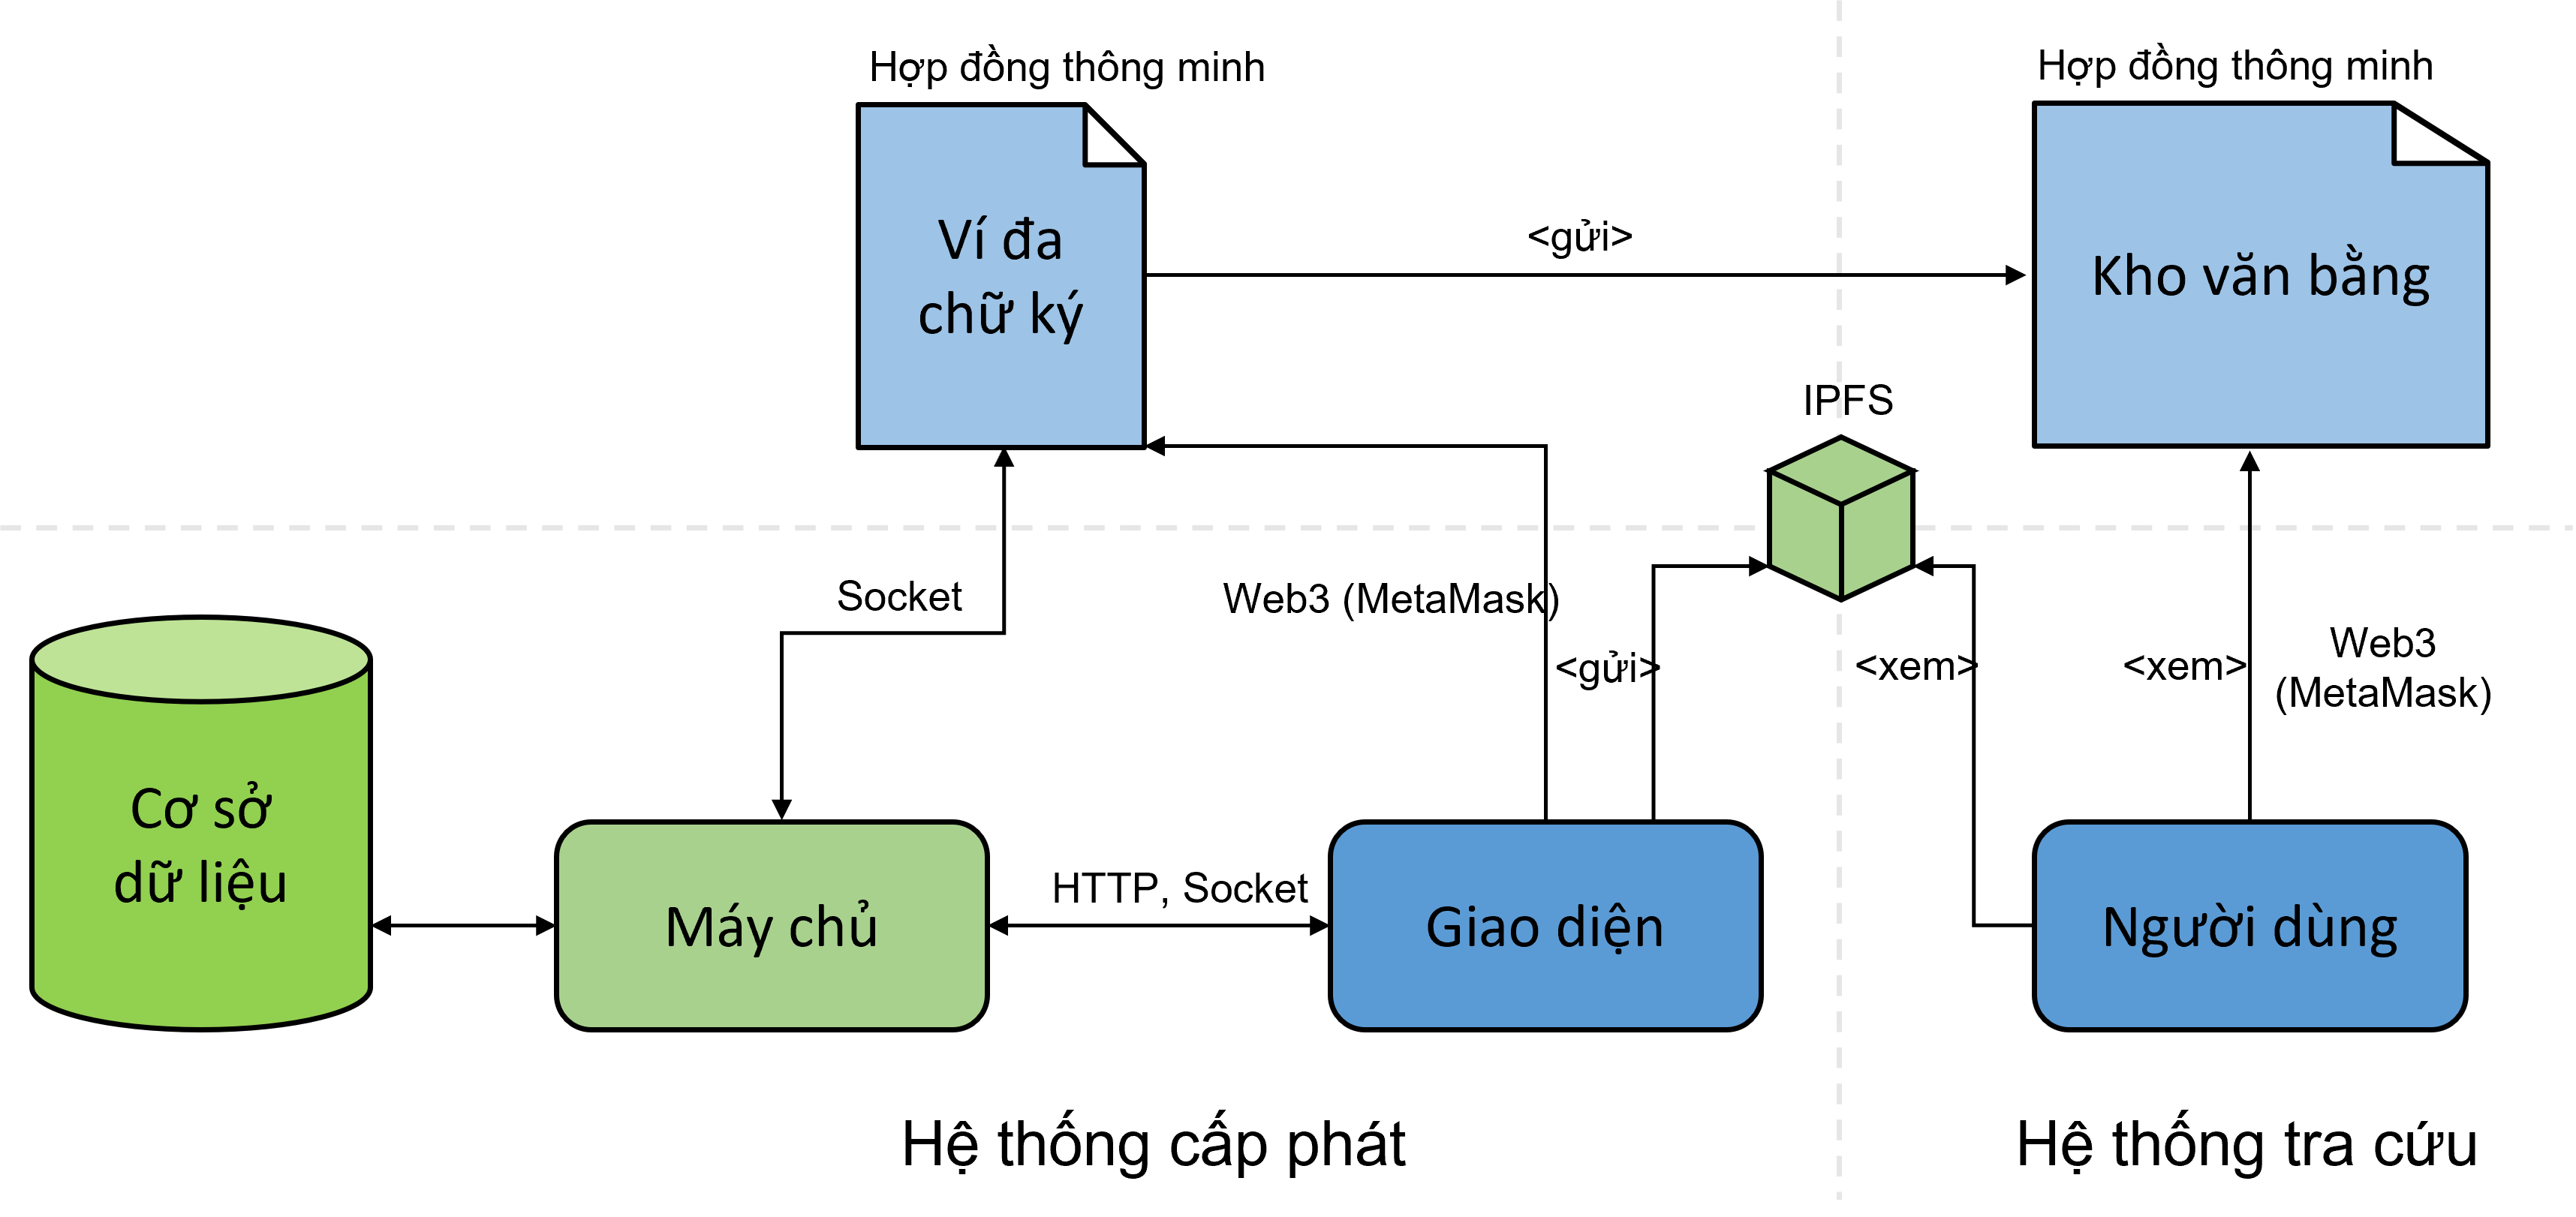
\includegraphics[width=400px]{anh/giai-phap/tong-quan-he-thong.png}
    \caption{Sơ đồ tổng quan các hệ thống và mạng chuỗi khối}
    \label{images/system-overview}
\end{figure}

Những hệ thống này sẽ tương tác với các hợp đồng thông minh trên mạng chuỗi khối, bao gồm \textit{Kho văn bằng} và \textit{Ví đa chữ ký}. Trong bài báo cáo này, em xin phép tập trung trình bày về phần thiết kế các hợp đồng thông minh được triển khai cùng hệ thống.


\subsection{Kho văn bằng}
\textit{Kho văn bằng} (hay \textit{kho chứng chỉ}) là một hợp đồng thông minh nắm giữ thông tin các văn bằng được lưu trữ trên mạng chuỗi khối. Thông tin được tổ chức theo cấu trúc dạng cây, mỗi mã số văn bằng trên mạng chuỗi khối sẽ tương ứng với các thông tin liên quan đến văn bằng đã được cấp phát.\\

Để lưu trữ văn bằng trên mạng chuỗi khối, các cơ sở giáo dục cần sử dụng một địa chỉ ví để tương tác với hợp đồng thông minh được triển khai trên mạng đó. Mỗi cơ sở phát hành văn bằng sẽ có một địa chỉ ví xác định, địa chỉ này sẽ được cơ quan như \textit{Bộ Giáo dục và Đào tạo} hoặc \textit{Chính phủ} ghi nhận là chữ ký đại diện cho cơ sở cấp phát văn bằng đó.\\

\begin{figure}[!ht]
    \centering
    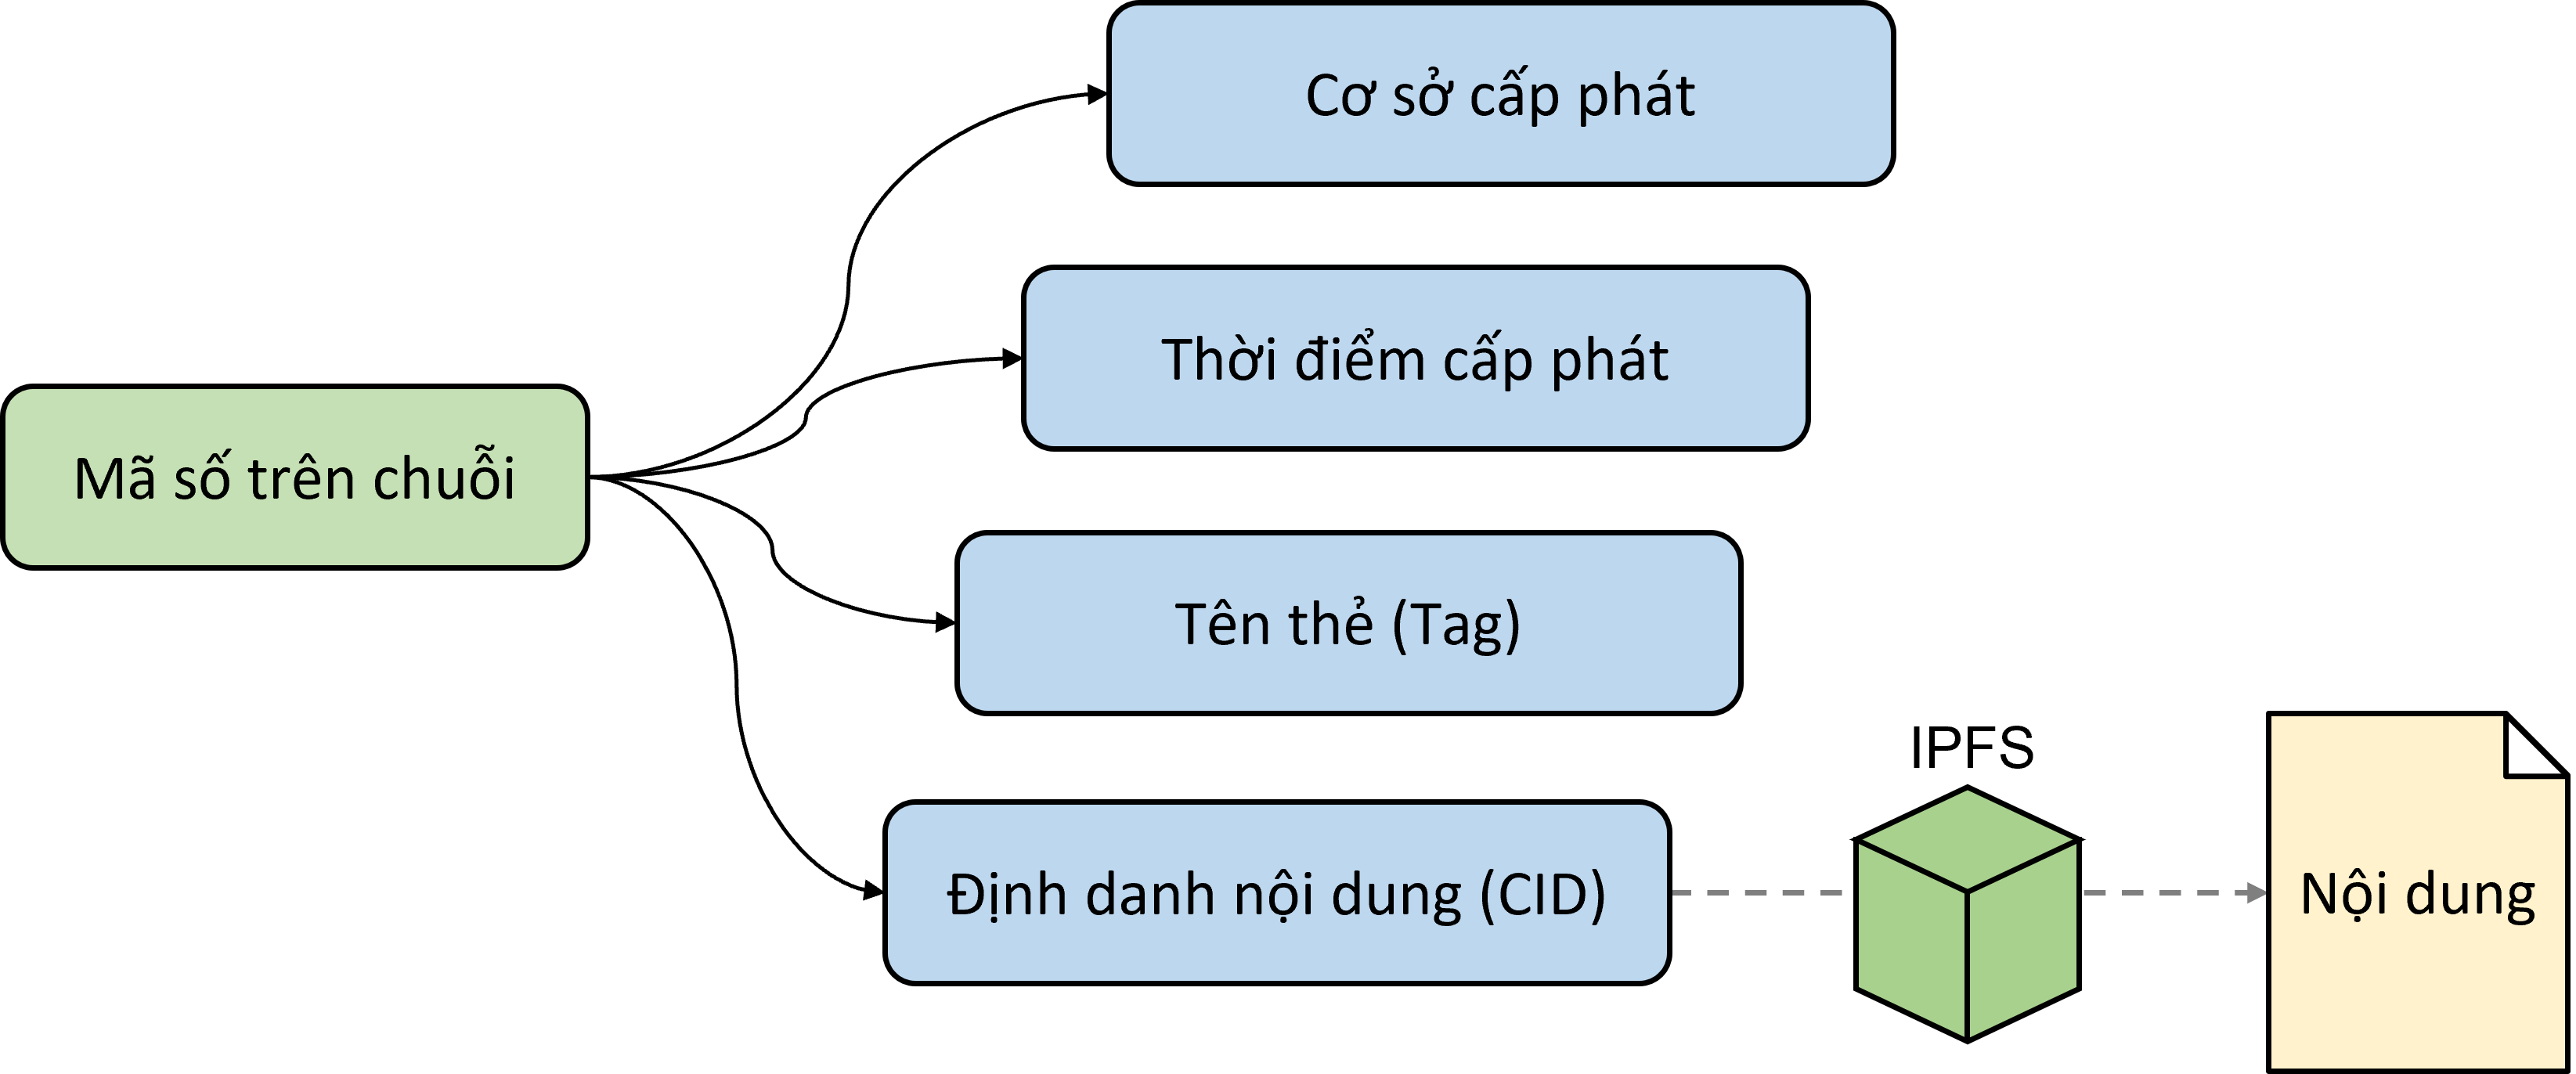
\includegraphics[width=400px]{anh/giai-phap/cau-truc-du-lieu.png}
    \caption{Cấu trúc lưu trữ thông tin trong \textit{kho văn bằng}}
\end{figure}

\textit{Kho văn bằng} cung cấp một số chức năng liên quan đến lưu thông tin, tra cứu thông tin văn bằng, phụ lục văn bằng, thông tin của các cơ sở giáo dục, tổ chức cấp phát văn bằng, chứng chỉ. Cụ thể, ba chức năng hiện có ở đây là:
\begin{itemize}
    \item Lưu thông tin văn bằng
    \item Xem thông tin văn bằng
    \item Khoá văn bằng
\end{itemize}

Đối với việc \textit{lưu thông tin}, địa chỉ ví của cơ sở (hay người) gửi yêu cầu lưu thông tin văn bằng sẽ được lấy làm \textit{Cơ sở cấp phát}, và thông tin đi kèm sẽ được sử dụng làm \textit{Tên thẻ} cho văn bằng. Như vậy, sẽ không có tình huống một cơ sở giáo dục phát hành văn bằng với địa chỉ của cơ sở khác, trường hợp nhầm lẫn do vô ý hoặc có chủ đích không thể xảy ra.\\

Để \textit{xem thông tin}, người tra cứu chỉ cần cung cấp mã số văn bằng đã được cấp phát. Những thông tin được hợp đồng thông minh trả về bao gồm cả định danh nội dung trên mạng IPFS, hệ thống tra cứu sẽ tự động lấy nội dung văn bằng (bao gồm cả phụ lục văn bằng) dựa trên định danh này.\\

Đối với trường hợp văn bằng đã được cấp phát nhưng thông tin bị sai hoặc không phù hợp, phía cơ sở cấp phát văn bằng có thể lựa chọn \textit{khoá văn bằng} lại. Người tra cứu không thể \textit{xem thông tin} đối với những văn bằng đã bị khoá.


\subsection{Ví đa chữ ký}
\textit{Ví đa chữ ký} là một hợp đồng thông minh với mục đích tăng tính bảo mật cho quá trình tương tác thay đổi thông tin văn bằng trên chuỗi khối.\\

Với việc "đẩy" thông tin văn bằng lên mạng chuỗi khối một cách thông thường, mỗi cơ sở giáo dục sử dụng địa chỉ ví của một cá nhân đại diện để tương tác, hoặc lựa chọn một địa chỉ ví và sử dụng chung cho cá nhân trong cơ sở. Điều này đảm bảo mỗi cơ sở cấp phát chứng chỉ có một địa chỉ duy nhất. Tuy nhiên, khi nhiều cá nhân cùng dùng một địa chỉ ví, khả năng mất cắp tài sản liên kết với địa chỉ này càng lớn, đặc biệt khi nó còn được sử dụng trong các giao dịch khác có giá trị về tài chính (như địa chỉ sở hữu tiền mã hoá với giá trị cao trên các \textit{sàn giao dịch}\footnote{Exchange}, hay liên kết với các \textit{DApp} khác). Do đó, một cơ chế giúp giảm thiểu khả năng nhiều người cùng sở hữu một địa chỉ ví và có thể sử dụng địa chỉ ví để xác thực thông tin cơ sở cấp phát văn bằng là vô cùng cần thiết. \textit{Ví đa chữ ký} ra đời để giải quyết vấn đề này.\\

Không giống với các \textit{hệ thống xác thực đa chữ ký}\footnote{Multi-signature authentication system} khi ít nhiều phụ thuộc vào các cơ chế xác thực phức tạp, \textit{ví đa chữ ký} sử dụng các tính năng, lợi thế của hợp đồng thông minh và mạng chuỗi khối. Ở \textit{ví đa chữ ký}, mỗi hành động cần thực thi (ở đây là việc cấp phát văn bằng) yêu cầu một số lượng nhất định sự đồng ý từ cá nhân. Địa chỉ ví của các cá nhân này đã được thêm vào danh sách "thành viên" ngay từ khi hợp đồng thông minh này được triển khai, và họ được coi như các "cổ đông" của "doanh nghiệp" cấp phát văn bằng khi có "tiếng nói" trong các "hoạt động" ở đây. Mỗi cơ sở cấp phát văn bằng sử dụng một \textit{ví đa chữ ký} duy nhất, và địa chỉ của hợp đồng thông minh này đại diện cho địa chỉ ví của cả cơ sở đó. Các văn bằng cần được đẩy lên \textit{kho văn bằng} sẽ được một cá nhân trong cơ sở gửi lên "ví" này. Các thành viên khác trong cơ sở có thể xem thông tin các văn bằng được gửi lên, và đưa ra biểu quyết "đồng ý" hay "không đồng ý" trên hợp đồng thông minh. Khi số lượng sự đồng ý đạt ngưỡng nhất định (được thiết lập từ đầu), các văn bằng đó được đẩy lên "kho", và thông tin được lưu trữ trên mạng chuỗi khối.\\

\begin{figure}[!ht]
    \centering
    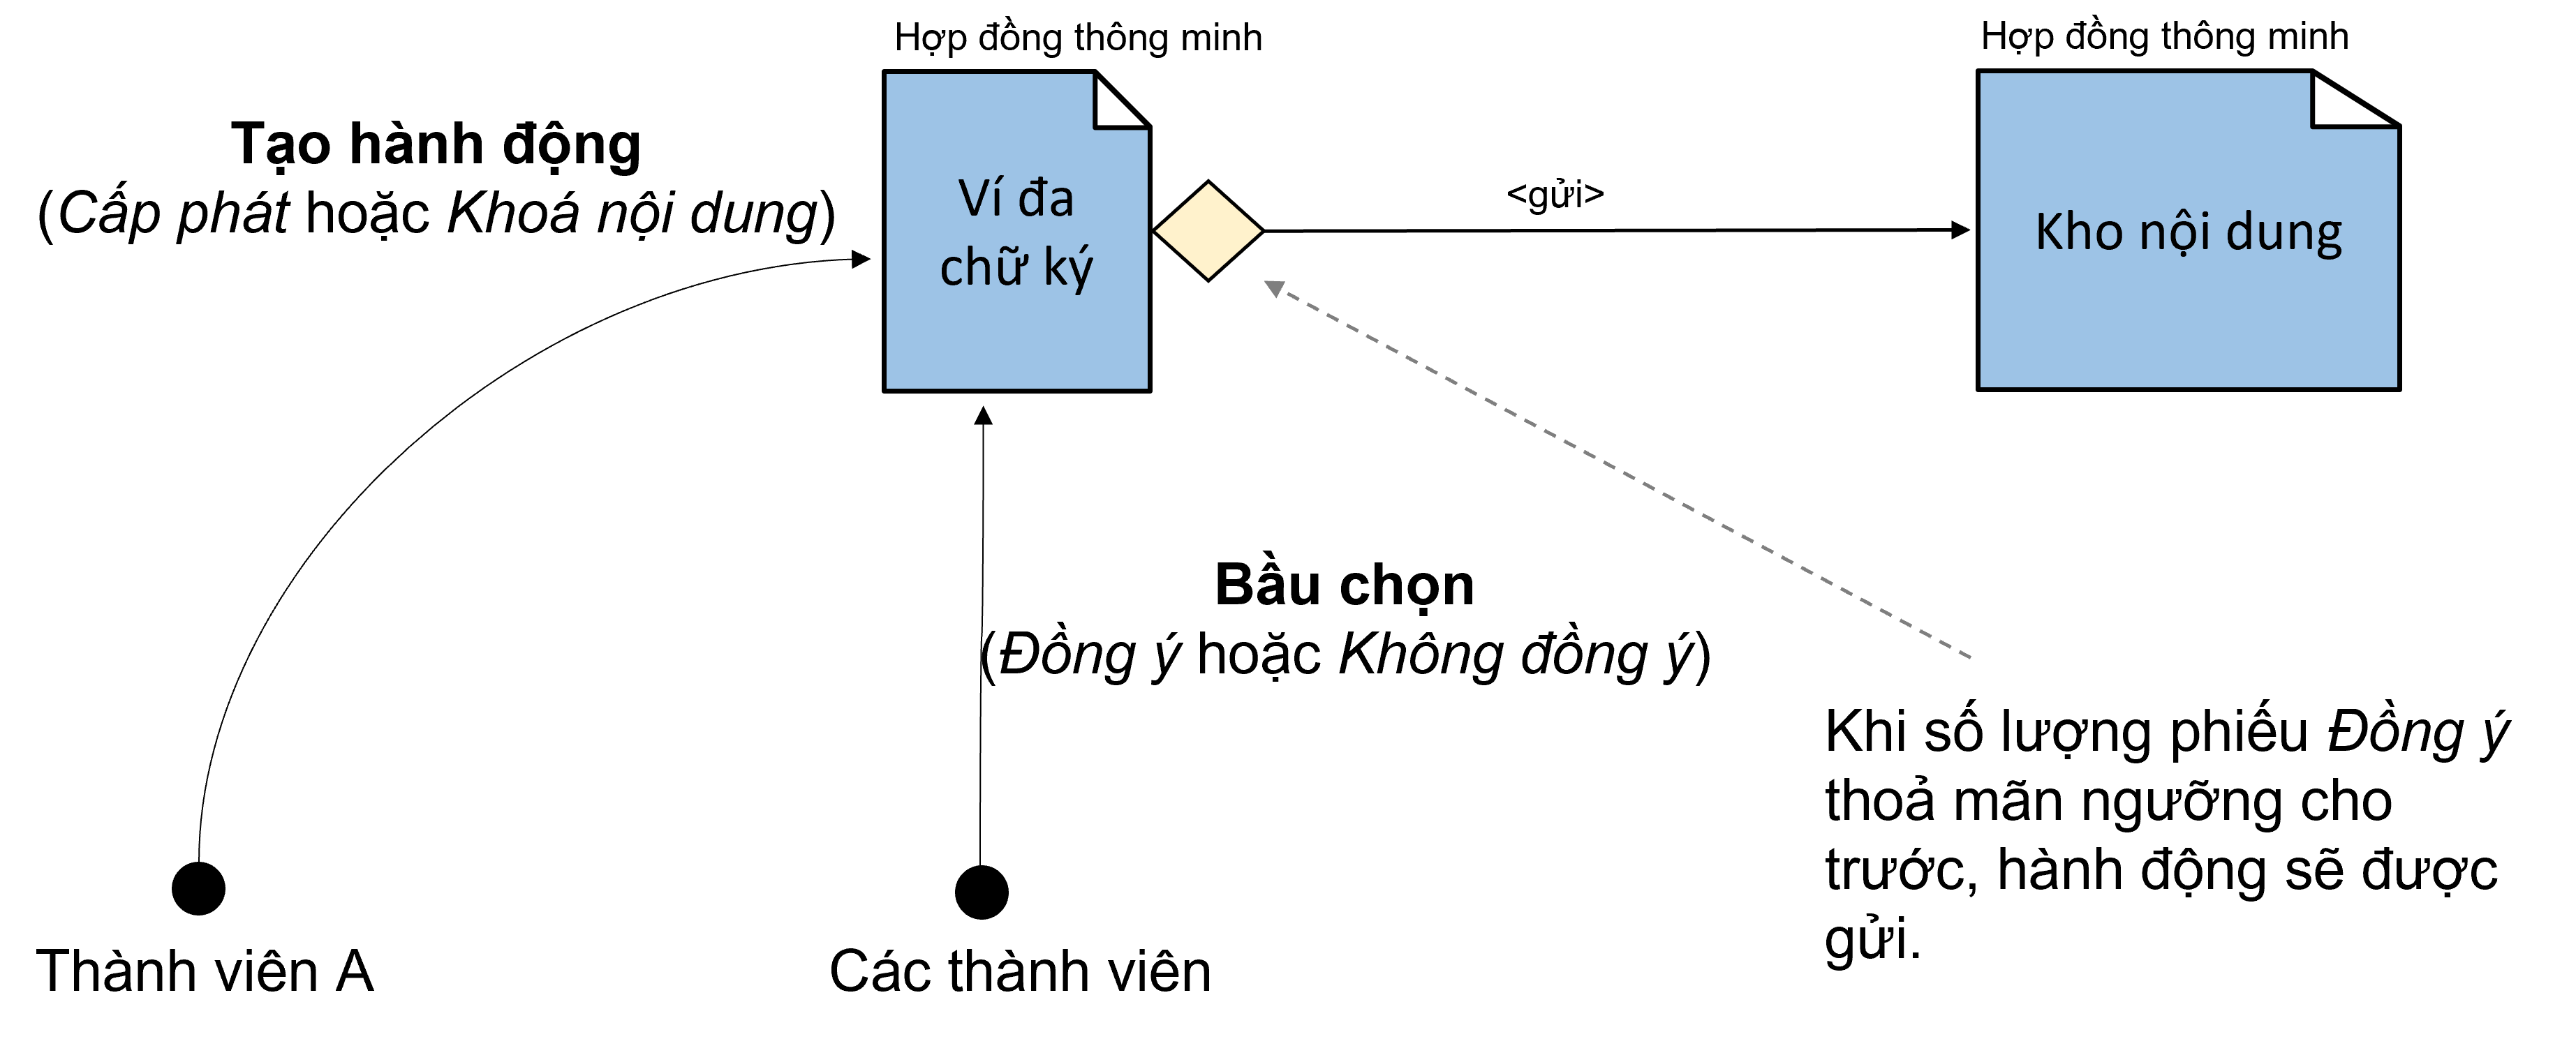
\includegraphics[width=400px]{anh/giai-phap/co-che-bau-chon.png}
    \caption{Cơ chế bầu chọn trong hệ thống}
\end{figure}


\subsection{Các yêu cầu liên quan}
Với \textit{hệ thống tra cứu}, không có có quá nhiều yêu cầu cần thực hiện. Hiện nay, các tiện ích, phần mềm được tạo ra, đáp ứng nhu cầu kết nối đến mạng chuỗi khối, trong số đó có thể kể đến \href{https://github.com/ChainSafe/web3.js}{\textit{Web3.js}}. \textit{Web3.js} là một dự án mã nguồn mở của \textit{ChainSafe}, được viết chủ yếu bởi ngôn ngữ lập trình \textit{JavaScript}, cung cấp các công cụ giúp người dùng tương tác với mạng Ethereum và các hợp đồng thông minh trên mạng này. \textit{Web3.js} có thể được tích hợp cho các \textit{DApp} dạng \textit{web}\footnote{Website} (webapp). Việc tra cứu thông tin văn bằng trở nên đơn giản và hết sức thân thiện, khi người dùng có thể trực tiếp thao tác qua giao diện trên trình duyệt.\\

\textit{Hệ thống cấp phát} cũng yêu cầu sử dụng cơ sở dữ liệu đơn giản để lưu trữ thông tin hành động (như cấp phát hay khoá văn bằng) trước khi chúng được thực thi trên mạng Ethereum. Ở đây, em sử dụng bảng \texttt{actions} với một số cột sau:
\begin{itemize}
    \item \texttt{id}: Định danh của hành động trên \textit{Ví đa chữ ký}, là số nguyên (tự động tăng trên hợp đồng thông minh), được sử dụng làm khoá chính cho bảng này.
    \item \texttt{executed}: Trạng thái thực thi của hành động, mang giá trị \texttt{true} (đã thực thi) hoặc \texttt{false} (chưa thực thi).
    \item \texttt{cancelled}: Trạng thái huỷ của hành động, mang giá trị \texttt{true} (đã bị huỷ) hoặc \texttt{false} (chưa bị huỷ).
\end{itemize}

Đồng thời, thông tin của quá trình bầu chọn cũng cần được ghi lại, tránh trường hợp một người bầu chọn nhiều lần cho một hành động (trường hợp này cũng không thể xảy ra do hợp đồng thông minh cũng đã kiểm tra các điều kiện phù hợp trước khi một người tham gia bầu chọn). Bảng \texttt{votes} được thiết kế cho việc này, bao gồm:
\begin{itemize}
    \item \texttt{action}: Định danh cho hành động được bầu chọn.
    \item \texttt{voter}: Địa chỉ hay định danh của người bầu chọn.
    \item \texttt{affirmed}: Trạng thái đồng tình của người bầu chọn, mang giá trị \texttt{true} nếu người đó đồng ý với hành động, ngược lại là \texttt{false}.
\end{itemize}

Cuối cùng chính là thông tin các văn bằng. Bảng \texttt{contents} được thiết kế cho phần này:
\begin{itemize}
    \item \texttt{id}: Mã số văn bằng trên \texttt{Kho văn bằng}, là số nguyên (tự động tăng trên hợp đồng thông minh).
    \item \texttt{cid}: Định danh nội dung hay địa chỉ nội dung của văn bằng trên mạng IPFS.
    \item \texttt{tag}: Chuỗi khác rỗng, được sử dụng cho mục đích tra cứu nội bộ và để ánh xạ giữa văn bằng trên hợp đồng thông minh với cơ sở dữ liệu. Trường này thường được gán giá trị bởi mã số học viên.
\end{itemize}

Ngoài ra, thông tin các thành viên được phép tham gia vào quá trình bầu chọn cũng như những thiết lập khác liên quan đến mạng Ethereum đều được lưu trữ trong cơ sở dữ liệu. Và ta cũng cần lưu ý rằng, phía máy chủ sẽ tự động cập nhật thông tin từ hợp đồng thông minh vào cơ sở dữ liệu; người dùng chỉ có quyền đọc dữ liệu từ đây (không có thao tác ghi vào cơ sở dữ liệu từ phía người dùng, người dùng tương tác trực tiếp với hợp đồng thông minh qua giao diện).

